\chapter{Cuestionario Final}


\section{Hallar el número de niveles de voltaje distintos que están presentes un período de la señal
	en el archivo obtenido con la la tarjeta de adquisición de datos de National Instruments.
	¿Cómo se relaciona esto con la resolución de la conversión analógico digital de la tarjeta de
	adquisición de datos y la amplitud pico a pico de la señal adquirida?}

La recolección de datos fue llevada a cabo utilizando una tarjeta de adquisición de datos de modelo NI USB 6210 fabricada por National Instruments \ref{fig:tarjeta-ni-6219} obteniendo como salida de la misma un conjunto de datos en formato csv el cual contempla los niveles de voltaje con una resolución 14 bits para la digitalización de los datos con un cambio mínimo de sensibilidad de $\frac{2mv}{2^{14}-1} = 0.122\mu V$.

Los datos fueron recolectados utilizando dos modos de la tarjeta de adquisición de datos: modo diferencial y modo RSE considerando para esto los niveles contemplados entre los 156mV y los - 56mV. En este escenario particular, se optó por utilizar los datos adquiridos en modo RSE, debido a que se compara con una referencia común, que suele ser el suelo o tierra. Esto significa que cada señal se mide con respecto a la misma referencia de tierra.


% TODO: \usepackage{graphicx} required
\begin{figure}[h]
	\centering
	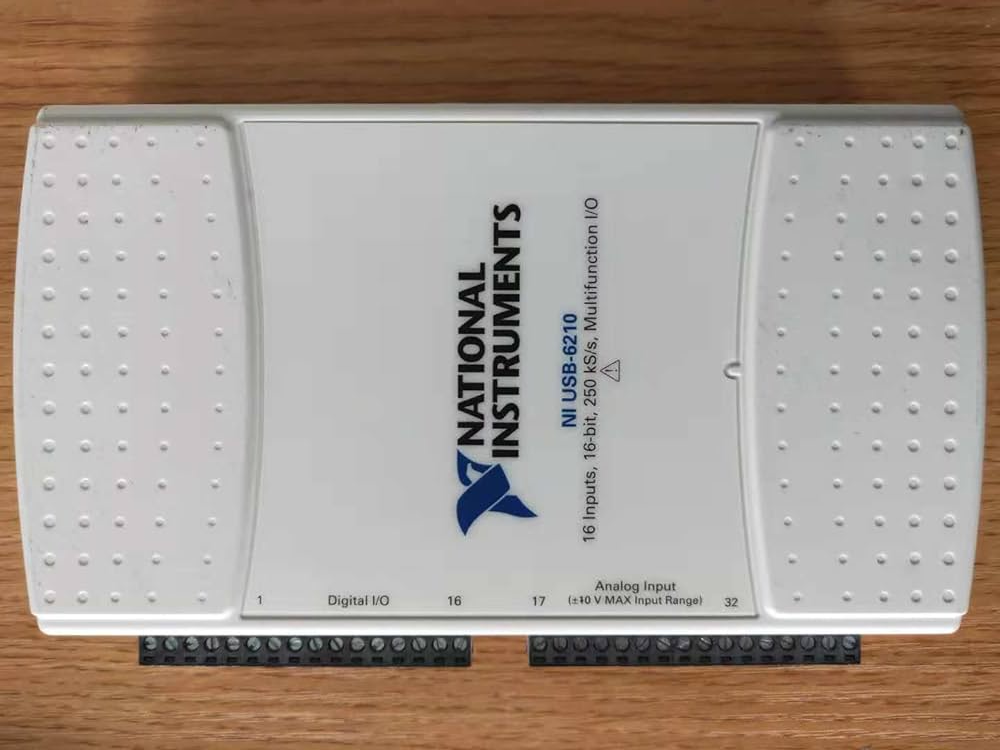
\includegraphics[width=0.6\linewidth]{media/tarjeta-ni-6219}
	\caption{Tarjeta de Adquisiciòn de datos NI USB 6210}
	\label{fig:tarjeta-ni-6219}
\end{figure}

\section{Procesamiento y filtrado de la señal}

En el procesamiento digital de señales biomédicas para el ruido mostrado en la figura \ref{fig:senal-ruido}, el filtrado es una etapa fundamental para mitigar las contaminaciones presentes en las señales adquiridas. En el contexto de un electrocardiograma (ECG), ruidos de alta frecuencia como la interferencia electromagnética o la actividad muscular (EMG) pueden enmascarar características clínicamente relevantes, como las ondas P, QRS y T segùn se menciona en \cite{valentinuzzi2004}. La metodología presentada aborda este problema implementando un filtro Butterworth pasabajo de cuarto orden con una frecuencia de corte de 30 Hz, aplicado a una señal de ECG muestreada a 1000 Hz. La elección del filtro Butterworth se justifica por su respuesta maximálmente plana en la banda pasante, lo que preserva la morfología de la señal sin introducir ondulaciones que podrían distorsionar la interpretación clínica, como se describe en \cite{butterworth_ecg}

La aplicación del filtro mediante \texttt{filtfilt(b, a, amp\_ecg)} introduce una mejora crítica para el análisis de bioseñales y cuyo resultado se muestra en la figura \ref{fig:senal-filtrada} y que a diferencia del filtrado causal convencional que introduce desfases temporales, esta técnica procesa la señal bidireccionalmente eliminando cualquier distorsión en la localización temporal de los eventos cardíacos. . 

El filtro, diseñado con frecuencia normalizada respecto a Nyquist:
\begin{equation}
	w_n = \frac{f_c}{f_s/2}
\end{equation}


\begin{figure}[h]
	\centering
	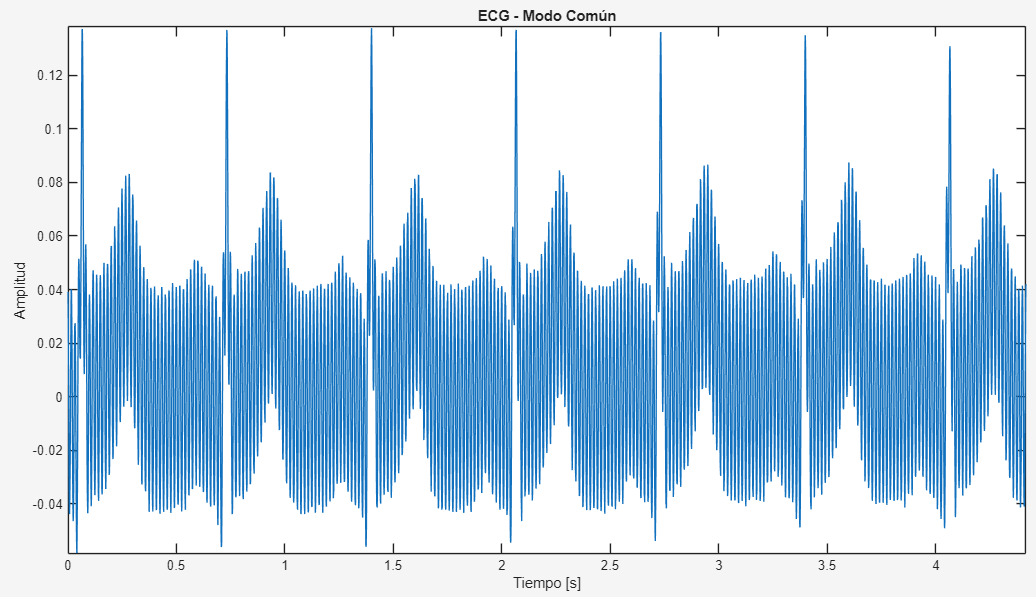
\includegraphics[width=0.6\linewidth]{media/senal-ruido}
	\caption{Señal ECG con ruido a 60Hz}
	\label{fig:senal-ruido}
\end{figure}

\noindent para $f_s = 1000$ Hz, atenúa eficazmente componentes superiores a 30 Hz mientras preserva la integridad morfológica de la señal ECG segmentada, demostrando su idoneidad para sistemas de monitoreo cardíaco y aplicaciones de análisis automático de bioseñales.

\begin{figure}[h]
	\centering
	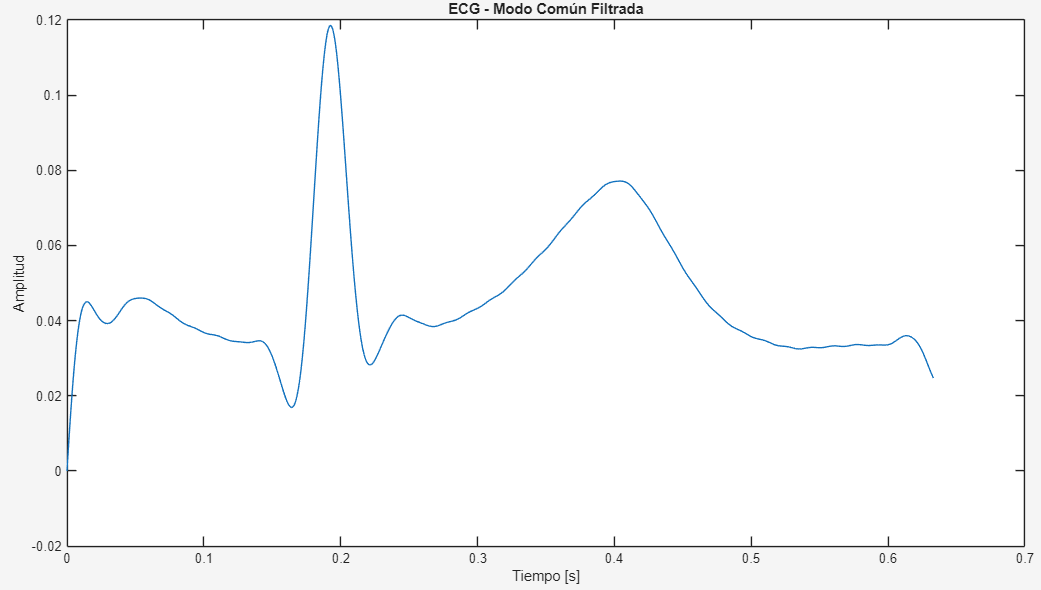
\includegraphics[width=0.6\linewidth]{media/senal-filtrada}
	\caption{Señal ECG filtrada}
	\label{fig:senal-filtrada}
\end{figure}

\section{Niveles de voltaje en la señal filtrada}

En la señal filtrada se pueden apreciar una reducción en los niveles de voltaje obtenidos para la señal ECG original con picos y valles en 156mV y los -56mV respectivamente en comparación con el pico en 83.77mv y el valle en -17.81mv como se muestra en la figura \ref{fig:niveles-voltaje-senal-filtrada} y cuyos valores se obtuvieron luego de restar los picos negativos que se sumaron para convertir dicha señal en una positiva para su escalado a 8bits.

\begin{figure}[h]
	\centering
	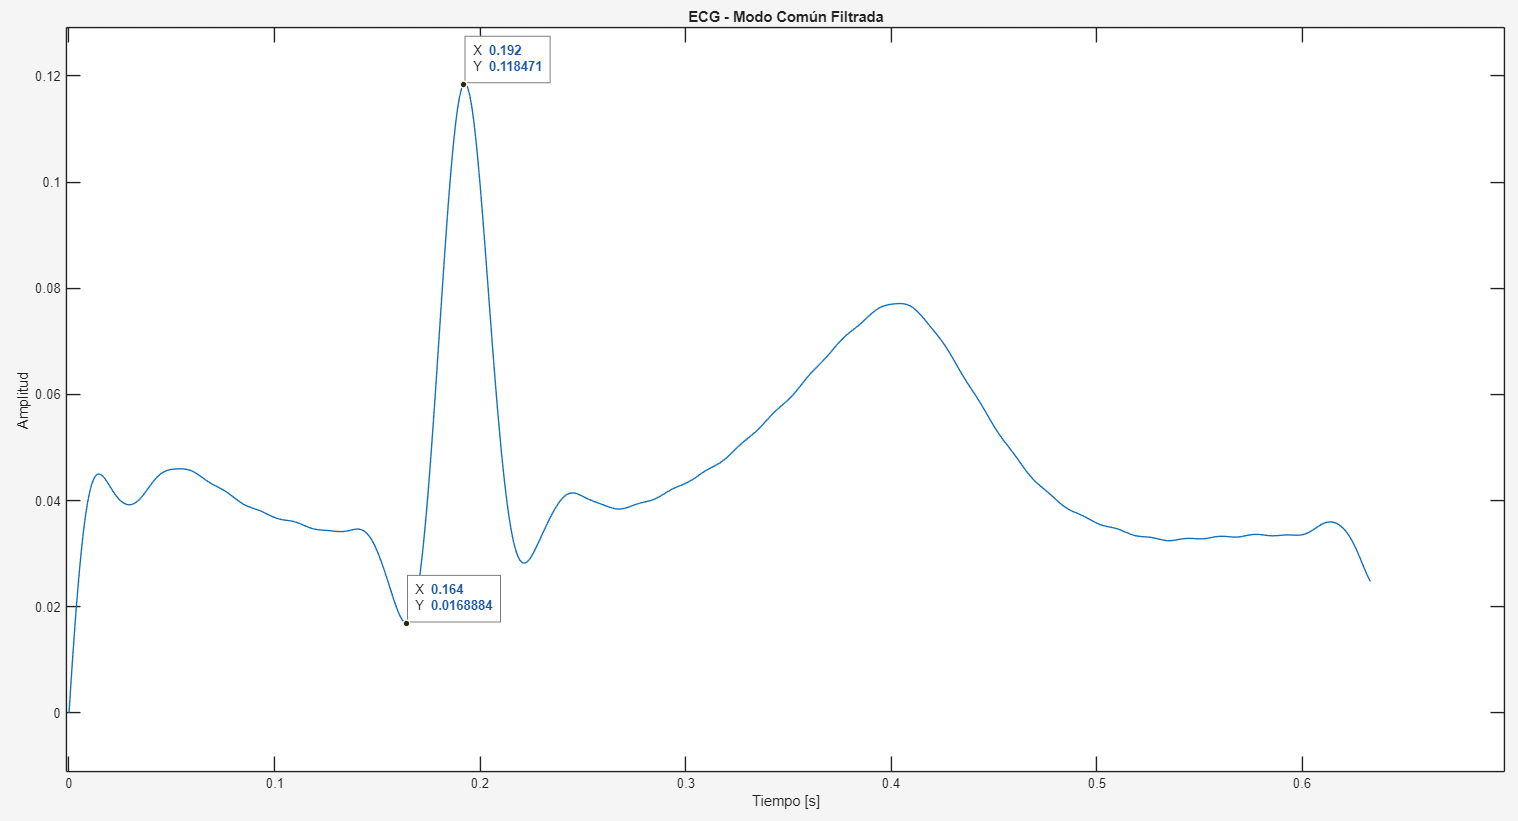
\includegraphics[width=0.6\linewidth]{media/niveles-voltaje-senal-filtrada}
	\caption{Niveles de voltaje en la señal ECG filtrada}
	\label{fig:niveles-voltaje-senal-filtrada}
\end{figure}

Apreciando una diferencia de $72.23mV$ y el cual se puede justificar con el filtrado del ruido a 60Hz proveniente de la señal alimentación eléctrica.

\section{Conversión de la señal filtrada a valores positivos de 8bits}

Para la conversión de la ECG digitalizada a una equivalente a una señal 8bits se hizo un escalado de la misma en función al pico máximo de la señal correspondiente 118.47mv luego de sumar a la señal en general el valor de 34.7mv para eliminar los valores negativos puesto que el ADC a emplear esta limitado a la conversión de valores positivos de voltaje.

\begin{figure}[h]
	\centering
	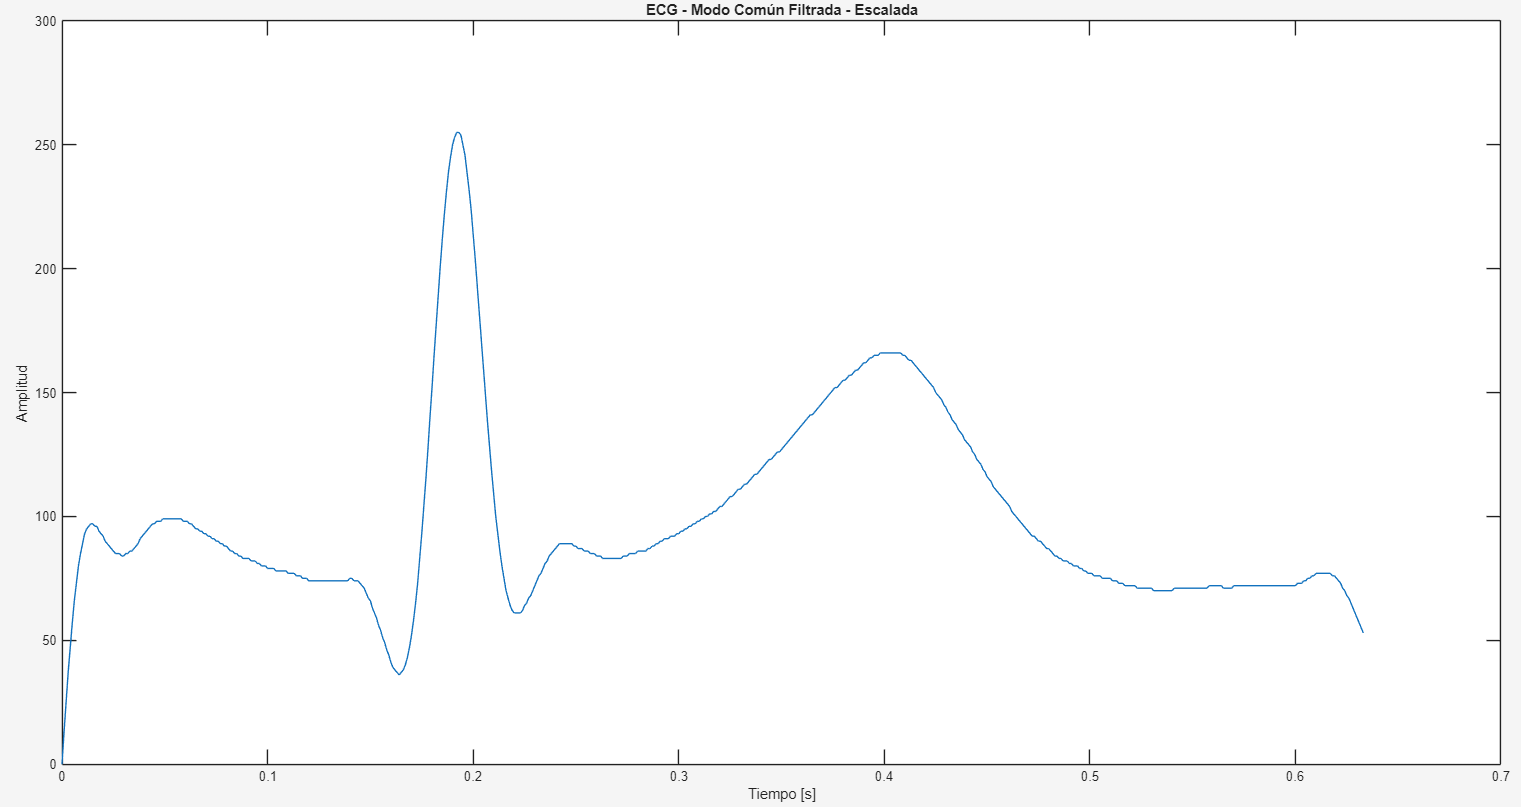
\includegraphics[width=0.6\linewidth]{media/senal-escalada}
	\caption{Señal ECG escalada a 8bits}
	\label{fig:senal-escalada}
\end{figure}

En la figura \ref{fig:senal-escalada} se aprecia la señal ECG escalada a 8 bits (valores entre 0 - 255) y la cual se obtuvo al modificar cada elemento del vector en MATLAB de la señal filtrada mediante el uso de una recta que representa un cambio lineal del escalado mediante la ecuación $y(x) = \frac{x*255}{0.1184}$ donde x representa un valor discreto de la señal.

\section{Describir con un diagrama de bloques y/o un circuito esquemático, la manera en que se
	implementó la conversión Digital/Analógica que tiene la resolución de 8 bits indicando los
	valores de los componentes y dispositivos utilizados.}

La conversión de la señal se realizo mediante la ejecución de diferentes pasos como su obtención, pre procesamiento, entre otros que se describe en la figura \ref{fig:diagrama-bloques} y que muestra un acercamiento general para la conversión realizada, sin embargo además de los pasos previos es necesario comprender el funcionamiento de la última etapa para la cual se hizo uso del microcontrolador ESP32.

\begin{figure}[h]
	\centering
	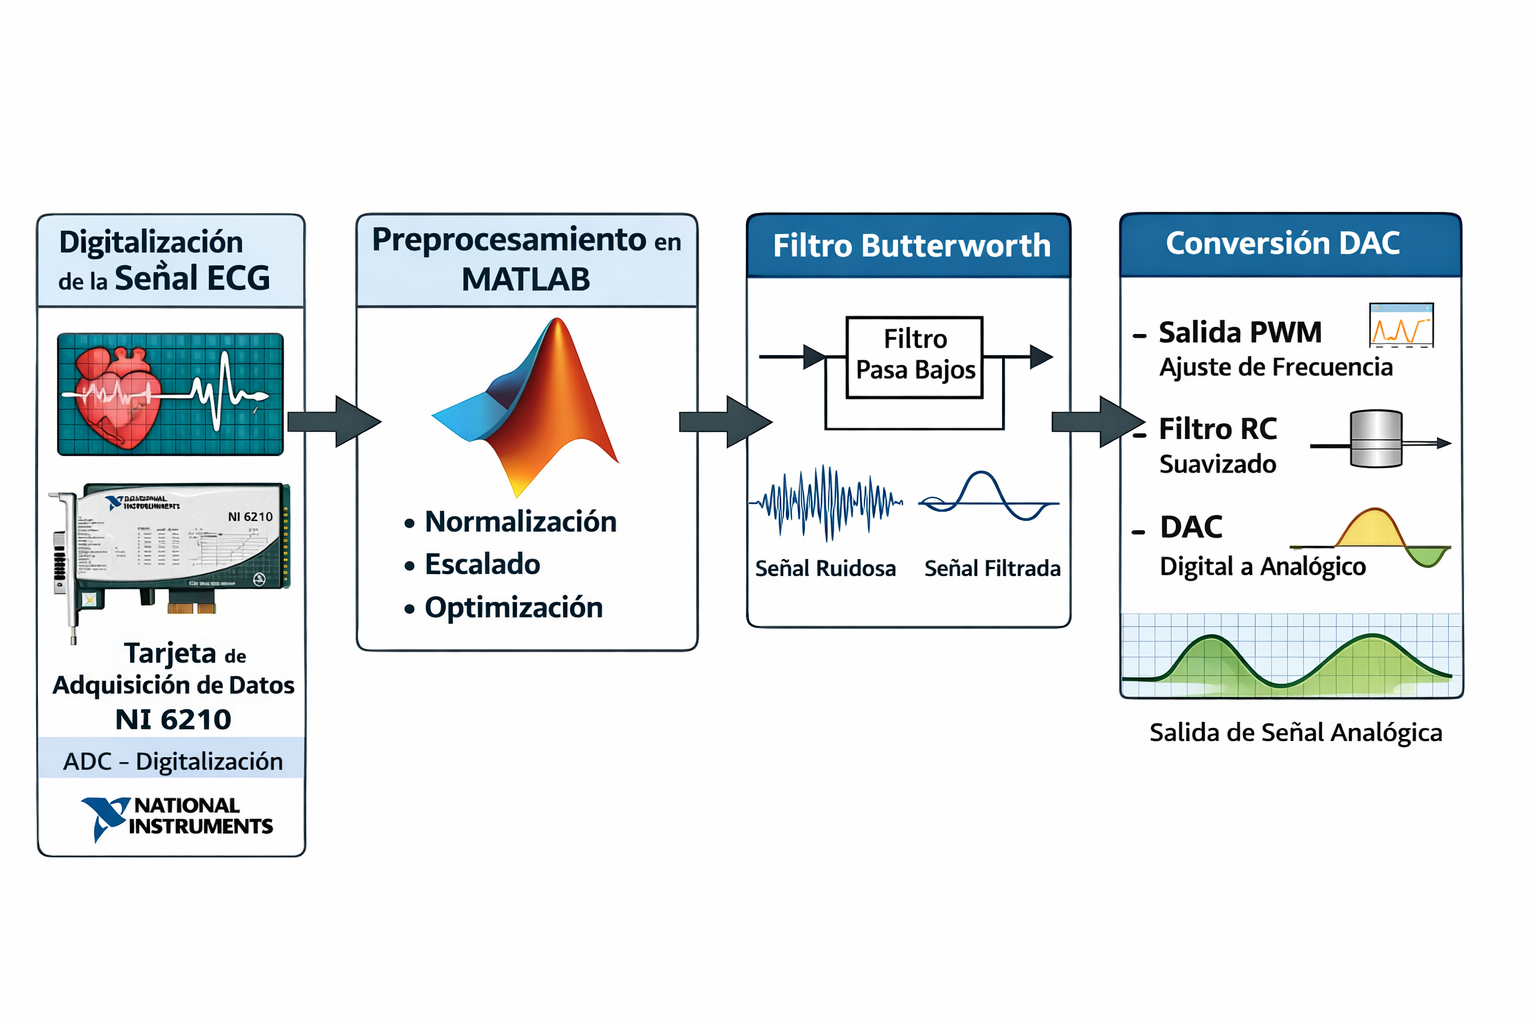
\includegraphics[width=0.6\linewidth]{media/diagrama-bloques}
	\caption{Diagrama de bloques para la conversión}
	\label{fig:diagrama-bloques}
\end{figure}

Y el cual se describe en la figura \ref{fig:diagrama-bloques-dac} que describe el flujo de datos desde la lectura del vector de información, su conversión de digital a analogica mediante el GPIO 25 que integra un DAC con valores entre los 0, 255.

\begin{figure}[h]
	\centering
	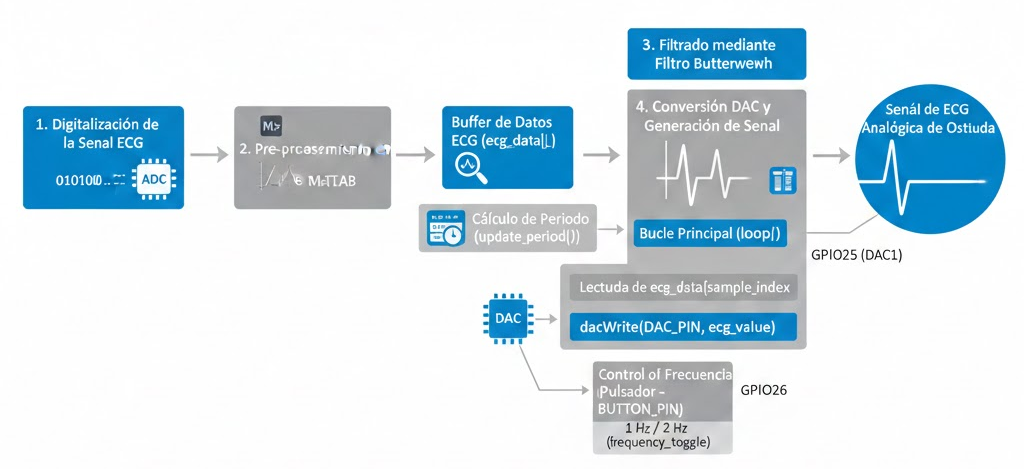
\includegraphics[width=0.7\linewidth]{media/diagrama-bloques-dac}
	\caption{Diagrama de bloques conversión D/A - ESP32}
	\label{fig:diagrama-bloques-dac}
\end{figure}

Implementando para ello código vital para el envío de la información en función a la frecuencia deseada modificable desde el GPIO 26 mediante un botón, cambiando esta de 60Hz a 120Hz.

\section{Indique el método de conversión D/A que ha elegido y describa los detalles y problemas
	que tuvo que resolver (incluyendo diseños de acondicionamiento de señal y filtros) para la
	conversión de tiempo discreto a tiempo continuo, así como los ajustes y/o cambios que
	tuvo que hacer para obtener la frecuencia en latidos por minuto deseada. Incluya un
	diagrama de bloques y un diagrama esquemático (circuito) del sistema electrónico
	implementado.}

Posterior a la etapa de adquisición y almacenamiento de la señal electrocardiográfica en formato digital, se empleó un microcontrolador ESP32 para realizar la conversión de la señal desde el dominio digital al dominio analógico. La selección de este microcontrolador se debe a que incorpora internamente dos canales de conversión digital--analógica (DAC), cada uno con una resolución de 8 bits, lo que permite convertir valores digitales comprendidos entre 0 y 255 en un voltaje analógico en el rango de 0 a 3.3~V.

En el presente trabajo se utilizó uno de los canales DAC disponibles del ESP32 para la generación de la señal electrocardiográfica analógica. A través de este canal, el microcontrolador envía de manera secuencial los valores digitales previamente procesados, reconstruyendo así la forma de onda del ECG en el dominio continuo. Este proceso permite emular el comportamiento temporal de una señal electrocardiográfica real, manteniendo la relación entre amplitud y tiempo de la señal original.

A continuación, se describe el procedimiento seguido para el acondicionamiento y la conversión de la señal electrocardiográfica digital a una señal analógica adecuada para su posterior visualización y análisis.


\subsection{Filtrado de la señal digital}

La señal electrocardiográfica digital fue inicialmente adquirida mediante el entorno de programación LabVIEW, el cual permite exportar los datos obtenidos a un archivo en formato Excel. No obstante, estos datos no pueden ser utilizados directamente por el microcontrolador, debido a la presencia de ruido y componentes no deseadas propias del proceso de adquisición.

Por esta razón, fue necesario realizar un procesamiento previo de la señal digital, el cual incluyó la aplicación de técnicas de filtrado digital con el objetivo de eliminar interferencias, como el ruido de la red eléctrica y otras perturbaciones de alta frecuencia. Este procesamiento previo garantiza que la señal cargada al microcontrolador represente de manera más fiel la actividad eléctrica cardíaca y evita distorsiones durante la conversión digital--analógica.

\begin{figure}[h]
	\centering
	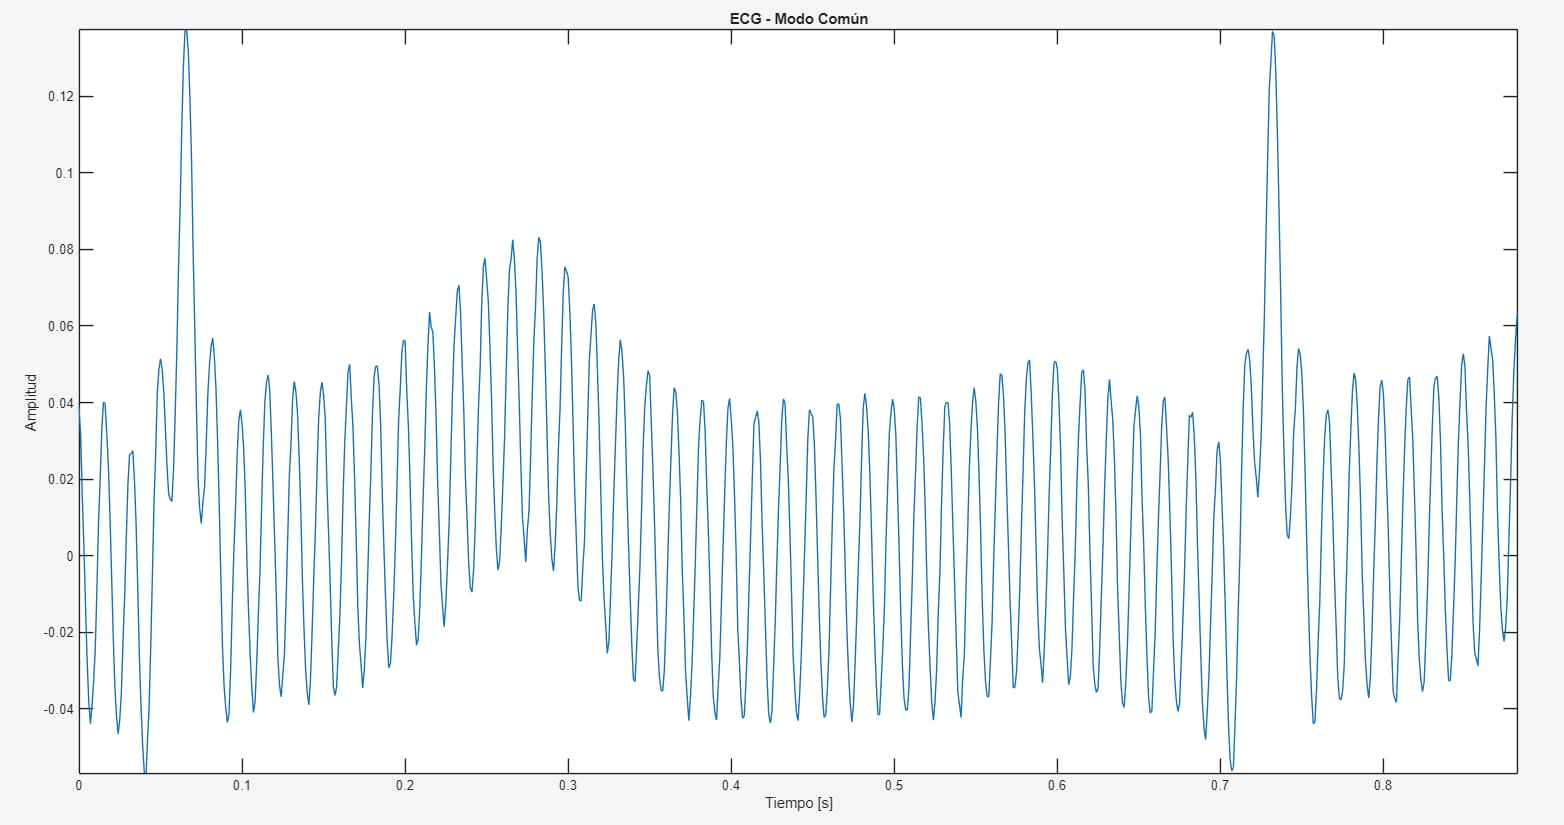
\includegraphics[width=0.6\linewidth]{media/señalconruido.png}
	\caption{Señal ECG con ruido}
	\label{fig:placeholder}
\end{figure}

\begin{figure}[h]
	\centering
	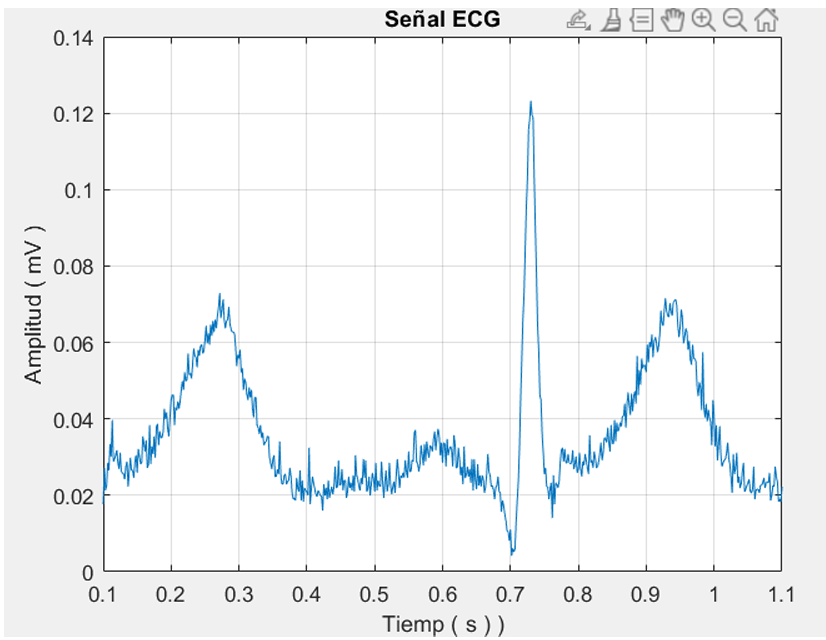
\includegraphics[width=0.6\linewidth]{media/Señal ECG para 1 ciclo.png}
	\caption{Señal ECG para un ciclo}
	\label{fig:placeholder}
\end{figure}

\begin{figure}[h]
	\centering
	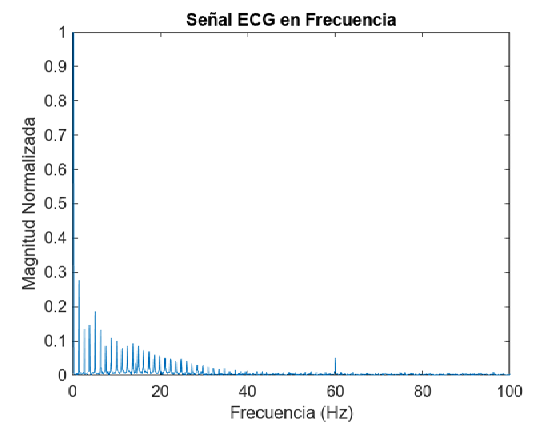
\includegraphics[width=0.6\linewidth]{media/fft.png}
	\caption{FFT de la señal ECG}
	\label{fig:placeholder}
\end{figure}

Se observa una componente que incorpora ruido a la señal y por ende debe se ser filtrada.

\newpage

\begin{minted}[
	fontsize=\footnotesize,
	linenos,
	frame=lines,
	breaklines
	]{matlab}
	
	clc, clear, close all;
	% Lectura del archivo de datos
	data_ecg = readmatrix("DATOS_ECG/ECG_ruido_common.csv");
	signal_ecg = data_ecg(:, 2);
	
	% Datos de lectura
	fs = 1000;
	ts = 1/fs;
	t = 0 : ts : (length(data_ecg(:, 1)) - 1)/fs;
	
	% Limitar la señal a 2 periodos de la señal
	limit_inf = 540;
	limit_sup = 1173;
	t2 = 0 : ts : (length(data_ecg(limit_inf:limit_sup, 1)) - 1)/fs;
	amp_ecg = data_ecg(limit_inf:limit_sup, 2);
	
	% Filtrado señal resultante
	fc = 30;
	wn = fc/(fs/2);
	[b, a] = butter(4, wn, 'low');
	ecg_low = filtfilt(b, a, amp_ecg);
	ecg_low = ecg_low + 0.01809 + 0.01661;
\end{minted}

\begin{figure}[h]
	\centering
	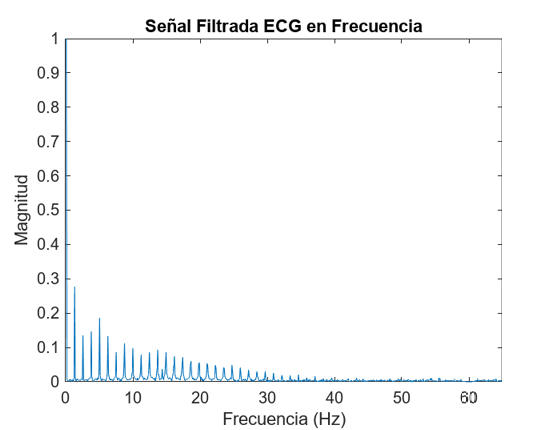
\includegraphics[width=0.6\linewidth]{media/señalfiltrada.png}
	\caption{Señal filtrada}
	\label{fig:placeholder}
\end{figure}

\begin{figure}[h]
	\centering
	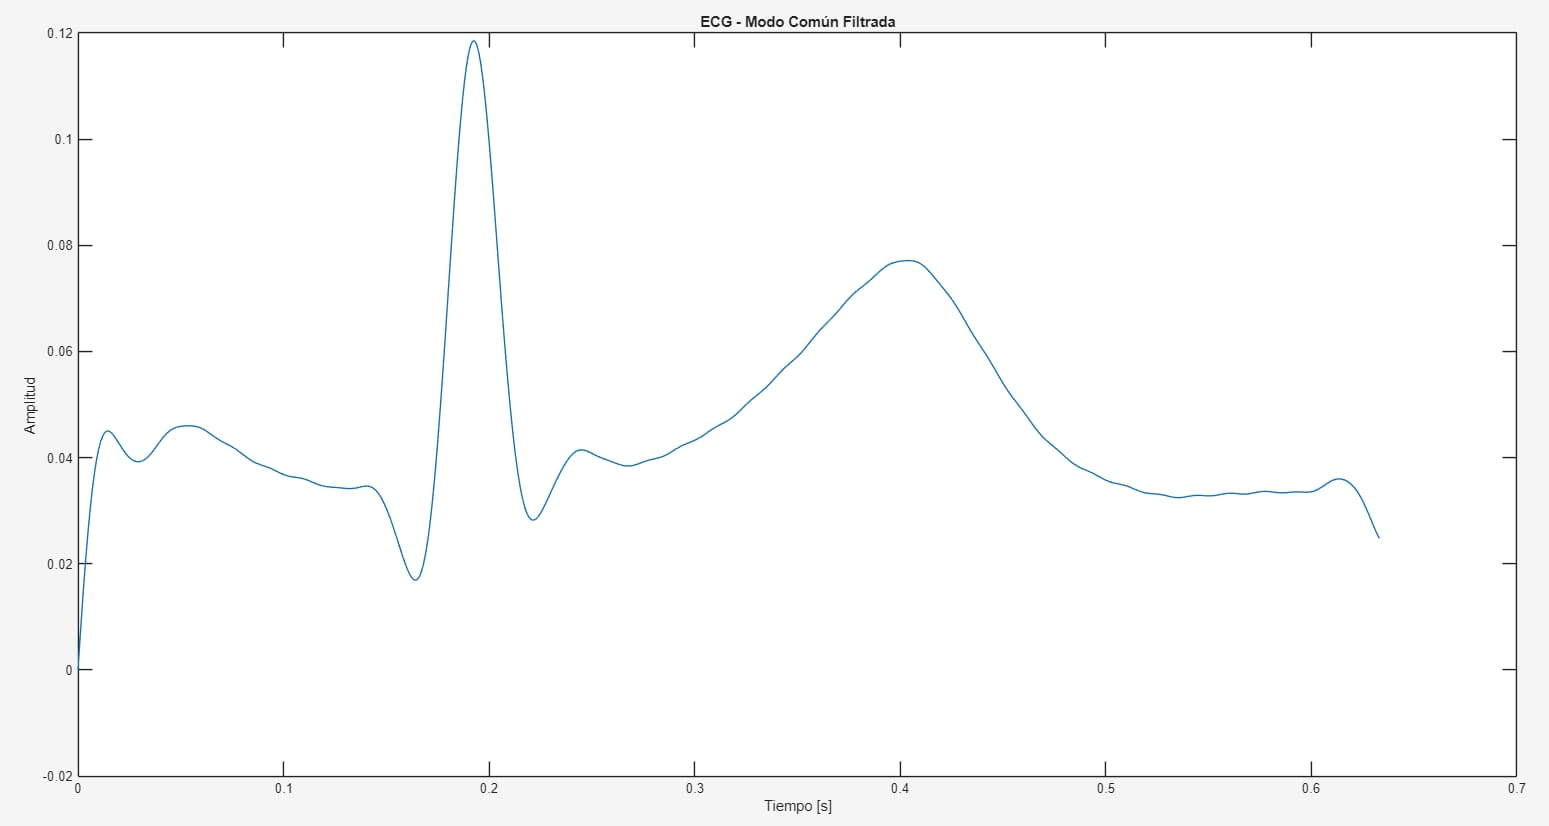
\includegraphics[width=0.6\linewidth]{media/señalconfiltro.png}
	\caption{Señal filtrada para un ciclo}
	\label{fig:placeholder}
\end{figure}


\subsection{Acondicionamiento de la señal digital}

Una vez aplicada la etapa de filtrado digital, la señal electrocardiográfica procesada es exportada desde el entorno MATLAB en formato de archivo Excel. Sin embargo, dado que el sistema de generación de la señal se implementa utilizando el entorno de desarrollo del microcontrolador (IDE de Arduino), resulta necesario realizar un acondicionamiento adicional de los datos digitales antes de su carga en el ESP32.

La señal electrocardiográfica original presenta una amplitud del orden de los milivoltios, con valores que no se encuentran directamente dentro del rango de operación del convertidor digital--analógico. De acuerdo con los datos obtenidos del archivo Excel, la señal presenta un valor 156~mV y $-56$~mV. Por tal motivo, se realizó un proceso de escalamiento de amplitud con el objetivo de adaptar la señal al rango digital requerido.

El acondicionamiento de la señal se llevó a cabo mediante los siguientes pasos:

\begin{enumerate}
	\item Se desplazó la señal restando el valor mínimo a todos los datos, de manera que el valor mínimo de la señal sea igual a cero.
	\item Posteriormente, se normalizaron los datos dividiéndolos entre la diferencia entre el valor máximo y el valor mínimo originales, logrando así llevar la señal al rango normalizado de 0 a 1.
	\item Una vez normalizada, la señal fue escalada multiplicando todos los valores por 1023, con el fin de adecuarla al rango digital de un convertidor de 10 bits.
	\item Finalmente, se eliminó la parte decimal de los valores obtenidos, redondeando los datos para obtener únicamente números enteros, los cuales pueden ser procesados correctamente por el microcontrolador.
\end{enumerate}

Este procedimiento permitió adaptar la señal electrocardiográfica digital a un formato compatible con el sistema de conversión digital--analógica, garantizando una correcta reconstrucción de la señal en el dominio analógico.


Adicionalmente, se incorporó una fila final en el archivo de datos para expresar los valores numéricos obtenidos en base decimal a su representación en base hexadecimal, formato que resulta compatible y de fácil interpretación para el microcontrolador durante la programación.

\subsection{Carga de los datos de la señal en el entorno Arduino}

Una vez acondicionada la señal electrocardiográfica digital, se procedió a cargar los datos en el entorno de desarrollo del microcontrolador utilizando el IDE de Arduino. Para ello, se seleccionó un conjunto de 800 muestras representativas de la señal ECG, cada una con una resolución de 8 bits. 

\subsection{Uso del DAC del ESP32 para la generación de la señal ECG}

El programa implementado en el ESP32 fue diseñado para procesar el arreglo de 687 datos de 8 bits y generar la señal analógica correspondiente mediante el uso de los convertidores digital-analógicos internos. Dado que el ESP32 únicamente dispone de salidas DAC con una resolución de 8 bits según \cite{esp32_dac}

Finalmente, la reconstrucción completa de la señal analógica equivalente a 8 bits de resolución se realiza externamente del microcontrolador a la placa de pruebas mediante el GPIO 25.



\begin{figure}[h]
	\centering
	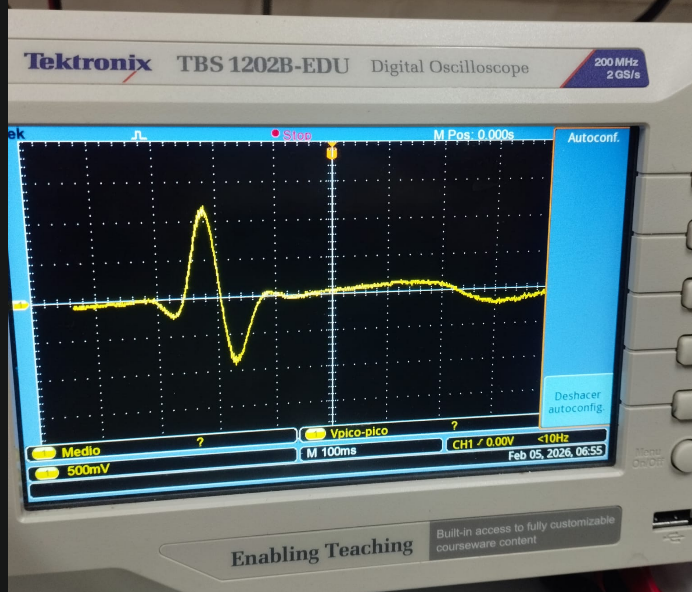
\includegraphics[width=0.6\linewidth]{media/salida de la señal.png}
	\caption{salida de la Señal en el osciloscopio}
	\label{fig:placeholder}
\end{figure}

\section{Diagrama y esquema del sistema}
El sistema implementado para la conversión de los datos electrocardiográficos desde el dominio digital al dominio analógico está compuesto por varias etapas funcionales. En una primera etapa, se emplea el microcontrolador ESP32, el cual se encarga de imprimir de manera secuencial los datos digitales de la señal ECG mediante el uso de su convertidor digital--analógico (DAC) interno.

Posteriormente, la señal analógica generada a la salida del DAC es aplicada a un filtro analógico paso bajo de segundo orden, cuyo objetivo principal es suavizar el comportamiento escalonado propio del proceso de conversión digital--analógica. Esta etapa de filtrado permite atenuar las componentes de alta frecuencia y obtener una señal más continua, logrando así una representación más fiel de una señal electrocardiográfica analógica.


\begin{figure}[h]
	\centering
	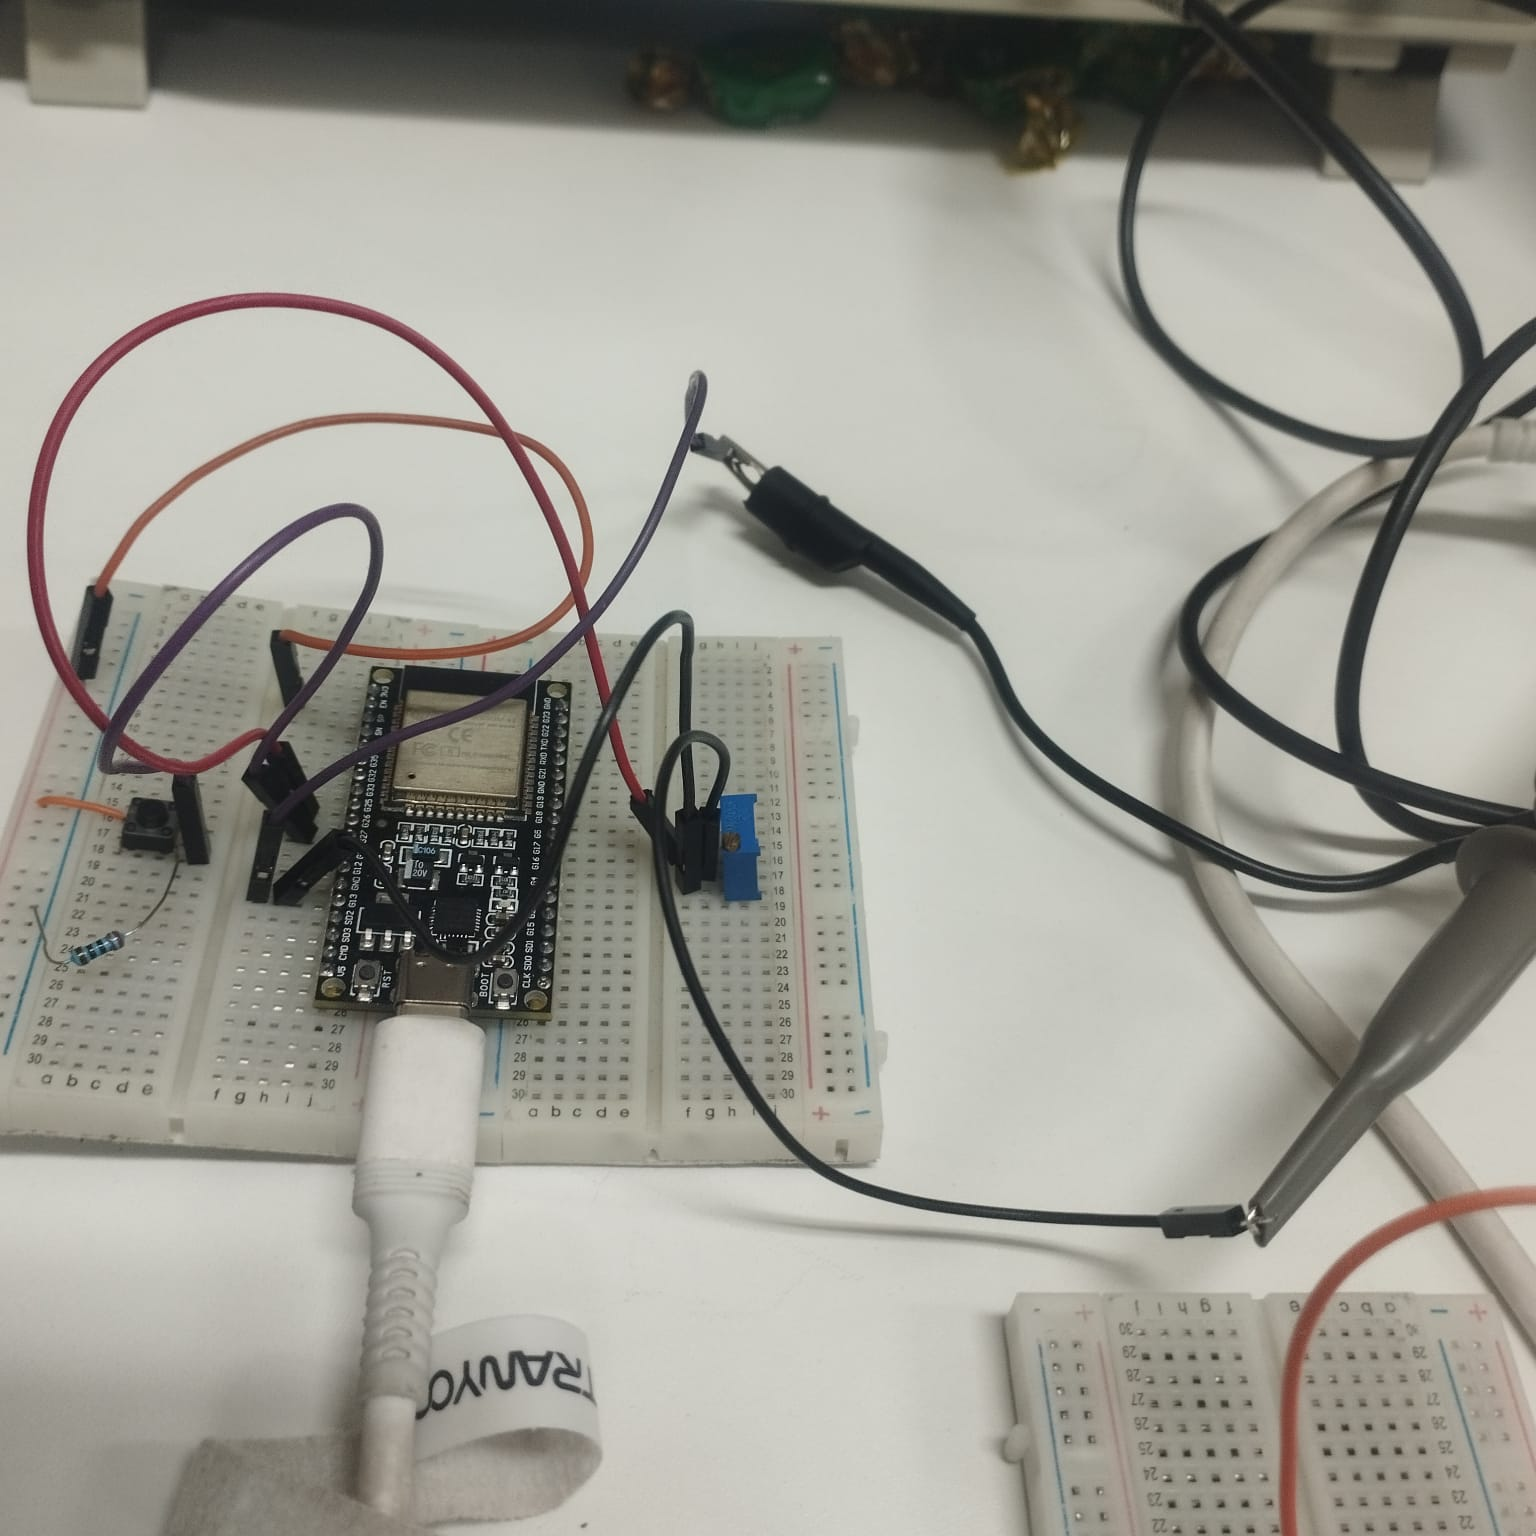
\includegraphics[width=0.6\linewidth]{media/circutioimplementado.png}
	\caption{Circuito Implementado}
	\label{fig:placeholder}
\end{figure}
\begin{figure}[h]
	\centering
	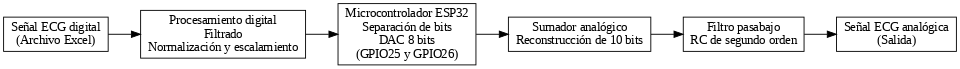
\includegraphics[width=0.8\linewidth]{media/digrama.png}
	\caption{Diagrama de bloques}
	\label{fig:placeholder}
\end{figure}


\section {Desarrolle y explique un diagrama de flujo del programa que se ejecuta en su microcontrolador o el sistema de desarrollo que haya utilizado.}

Para la generación de la señal electrocardiográfica analógica se desarrolló un programa utilizando el entorno de desarrollo Arduino IDE, el cual permite la programación de microcontroladores como el ESP32 de manera eficiente y accesible. La elección de este entorno se debe a su interfaz intuitiva y a la disponibilidad de librerías que facilitan la configuración de los periféricos internos del microcontrolador, como los convertidores digital--analógicos (DAC).

El programa implementado tiene como objetivo principal imprimir de manera secuencial los valores digitales previamente acondicionados de la señal electrocardiográfica, convirtiéndolos en señales analógicas a través de los DAC del ESP32. Para ello, el algoritmo sigue una estructura ordenada que inicia con la inicialización del microcontrolador y la configuración de los pines asociados a las salidas analógicas. Posteriormente, se cargan en memoria los arreglos de datos correspondientes a la señal ECG y se permite la selección de la frecuencia de latido mediante un pulsador.

Una vez seleccionada la frecuencia, el programa envía de forma secuencial cada muestra de la señal a las salidas DAC, aplicando un retardo controlado entre muestras para fijar la frecuencia de muestreo y, en consecuencia, la frecuencia cardíaca deseada. Durante este proceso, el índice que recorre el arreglo de datos se incrementa de manera progresiva y, al alcanzar el final del arreglo, se reinicia automáticamente, permitiendo la reproducción cíclica y continua de la señal electrocardiográfica.

A continuación, se presenta el diagrama de flujo que describe de manera gráfica la lógica de funcionamiento del programa desarrollado para el ESP32.

\begin{figure}[h]
	\centering
	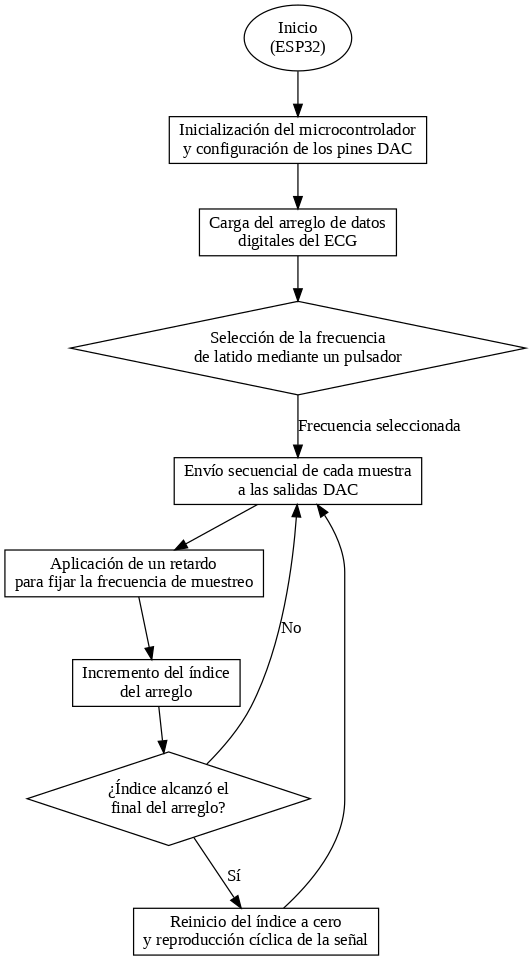
\includegraphics[width=0.5\linewidth]{media/diagramaflujo.png}
	\caption{Diagrama de Flujo}
	\label{fig:placeholder}
\end{figure}